% Order Flow Imbalance: standalone research note
% Compile from the report/ directory:  pdflatex OFI_Project_Report.tex
% (figures are pulled from ../results/figures/)
\documentclass[11pt]{article}

\usepackage[T1]{fontenc}
\usepackage{lmodern}
\usepackage[a4paper,margin=1in]{geometry}
\usepackage{graphicx}
\usepackage{booktabs}
\usepackage{array}
\usepackage{float}
\usepackage{caption}
\usepackage[hidelinks]{hyperref}

\graphicspath{{../results/figures/}{results/figures/}}

\captionsetup{font=small,labelfont=bf}
\setlength{\parskip}{6pt}
\setlength{\parindent}{0pt}
\renewcommand{\arraystretch}{1.25}
\newcolumntype{L}[1]{>{\raggedright\arraybackslash}p{#1}}

% Unnumbered, hanging-indent reference list (author-year style)
\newenvironment{reflist}{%
  \par\setlength{\parindent}{0pt}%
  \begin{list}{}{%
    \setlength{\leftmargin}{1.5em}%
    \setlength{\itemindent}{-1.5em}%
    \setlength{\itemsep}{3pt}%
    \setlength{\parsep}{0pt}%
    \setlength{\topsep}{4pt}%
  }%
}{\end{list}}

\begin{document}

\begin{center}
  {\LARGE\bfseries Order Flow Imbalance}\\[4pt]
  {\normalsize A microstructure study of OFI as a price-predictive signal}\\[6pt]
  {\normalsize Luke Yin}\\[2pt]
  {\small June 2026}
\end{center}
\vspace{4pt}

\section*{Summary}

Order Flow Imbalance (OFI) measures net buying versus selling pressure at the top of
the limit order book. Using 300{,}000 simulated book events (8.3 hours, roughly a
one-tick spread), this note finds that OFI explains a large share of contemporaneous
one-second price moves and retains some forecasting power out of sample, but the
predictable move is smaller than the spread, so a liquidity taker cannot trade it
profitably after costs. A market maker can use the same signal to skew quotes,
controlling inventory and improving its risk-adjusted return.

\begin{itemize}\setlength{\itemsep}{2pt}
\item OFI explains 53\% of contemporaneous one-second price moves ($R^2 = 0.53$,
      $t = 132$), or 88\% using the top five levels.
\item It forecasts the next second weakly (IC $= 0.18$) and holds out of sample
      (IC $= 0.19$).
\item The predicted move ($0.09$ ticks) is about 29 times smaller than the round-trip
      taker cost ($2.48$ ticks), so a cost-aware taker makes 0 trades.
\item Skewing Avellaneda-Stoikov quotes by OFI keeps inventory tightly bounded
      ($\pm 15$ versus $\pm 173$ for naive quoting) while recovering most of the PnL that
      plain inventory control gives up (\$110 versus \$18), the best risk-adjusted return
      of the three policies.
\end{itemize}

\section{Price impact}

A regression of the per-second mid-price change on OFI (Cont, Kukanov and Stoikov,
2014) gives $R^2 = 0.53$ ($t = 132$); the near-linear relationship is consistent with
Kyle-type linear price impact (Kyle, 1985). Using OFI from the top five book levels
(Xu, Gould and Howison, 2020) raises this to $R^2 = 0.88$.

\begin{figure}[H]
\centering
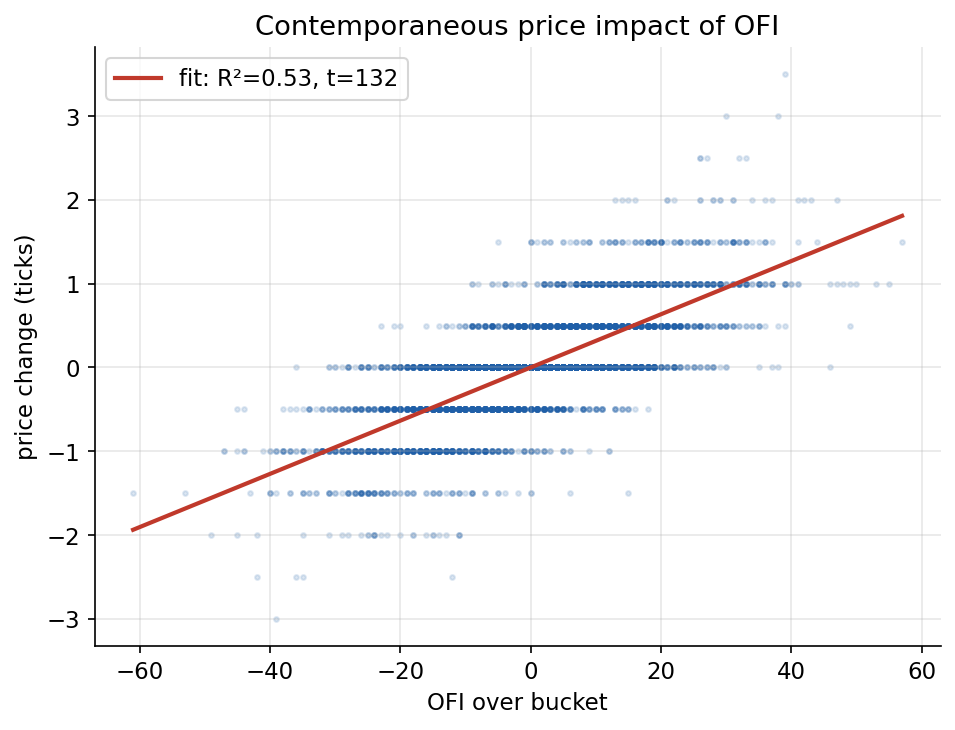
\includegraphics[width=0.72\linewidth]{03_impact_scatter.png}
\caption{Per-second price change versus OFI.}
\end{figure}

\begin{figure}[H]
\centering
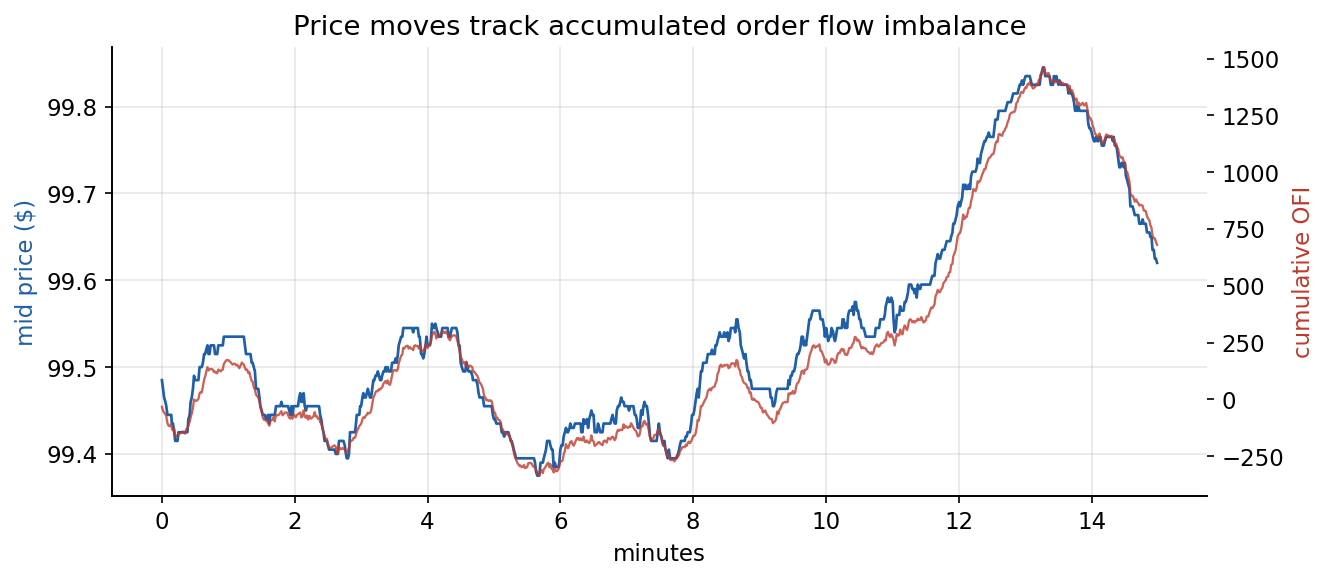
\includegraphics[width=\linewidth]{02_price_vs_ofi.png}
\caption{Mid price and cumulative OFI over a 15-minute window.}
\end{figure}

\section{Forecasting}

Forecasting the next move is weaker. The one-second information coefficient is
$0.18$ and holds out of sample (in-sample $0.18$, out-of-sample $0.19$ on a 70/30
chronological split). The IC rises with horizon, which indicates OFI predicts a
persistent drift rather than a single move.

\begin{figure}[H]
\centering
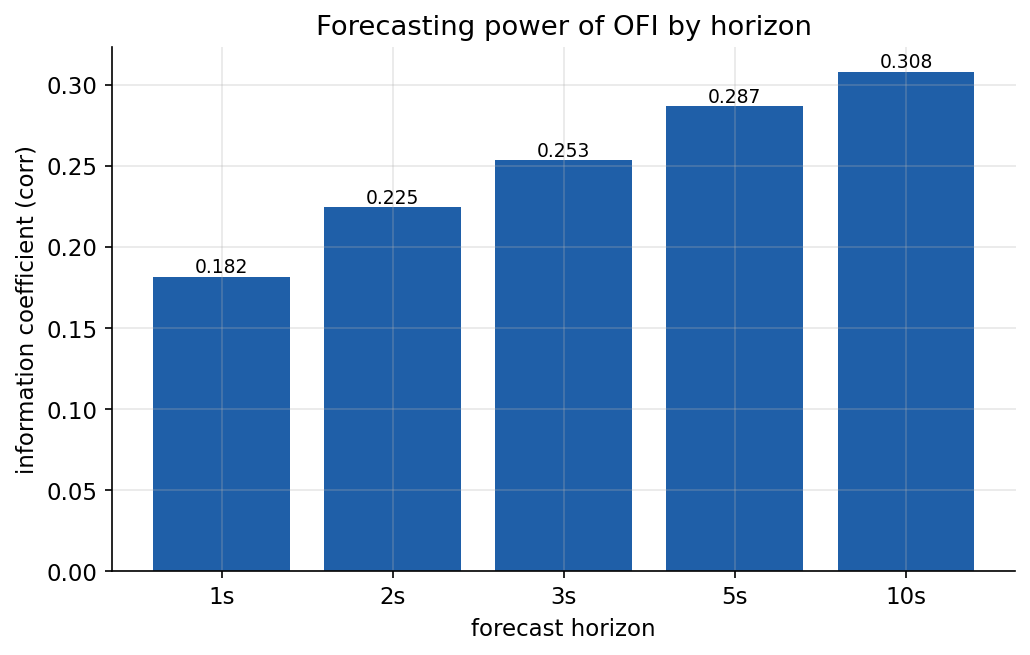
\includegraphics[width=0.8\linewidth]{04_forecast_decay.png}
\caption{Information coefficient by forecast horizon.}
\end{figure}

\section{Transaction costs}

The predicted next-second move averages $0.09$ ticks. A taker round trip costs about
$2.48$ ticks (two spread crossings plus fees), roughly 29 times the edge. Out of
sample the signal is positive gross ($+0.29$ ticks per trade) but negative net
($-2.20$ ticks per trade); a taker that trades only when the predicted edge exceeds
the cost makes 0 trades.

\begin{figure}[H]
\centering
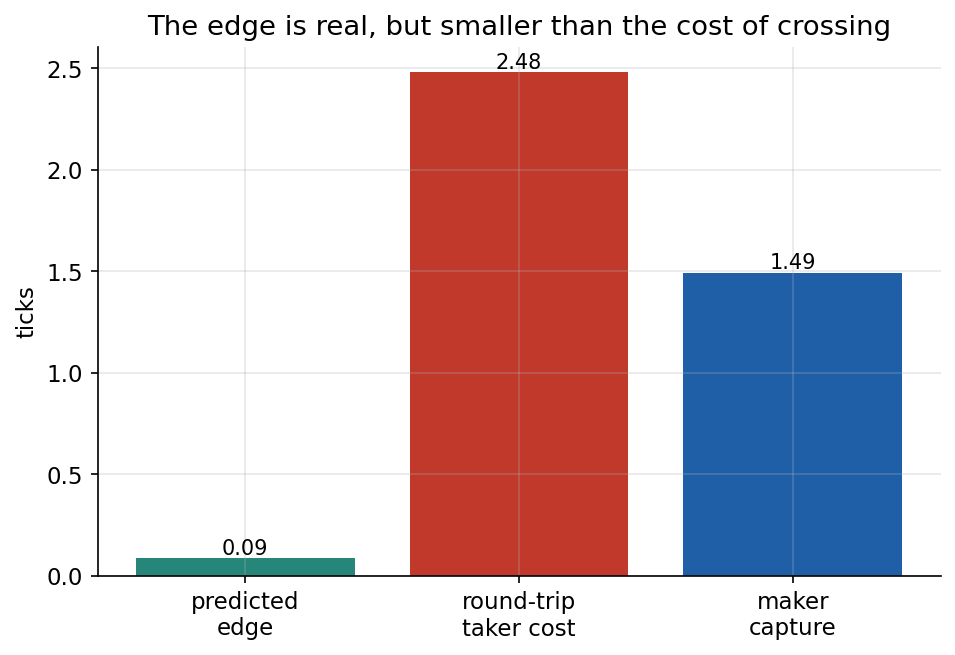
\includegraphics[width=0.72\linewidth]{05_edge_vs_cost.png}
\caption{Predicted edge, taker cost, and maker capture, in ticks.}
\end{figure}

\begin{figure}[H]
\centering
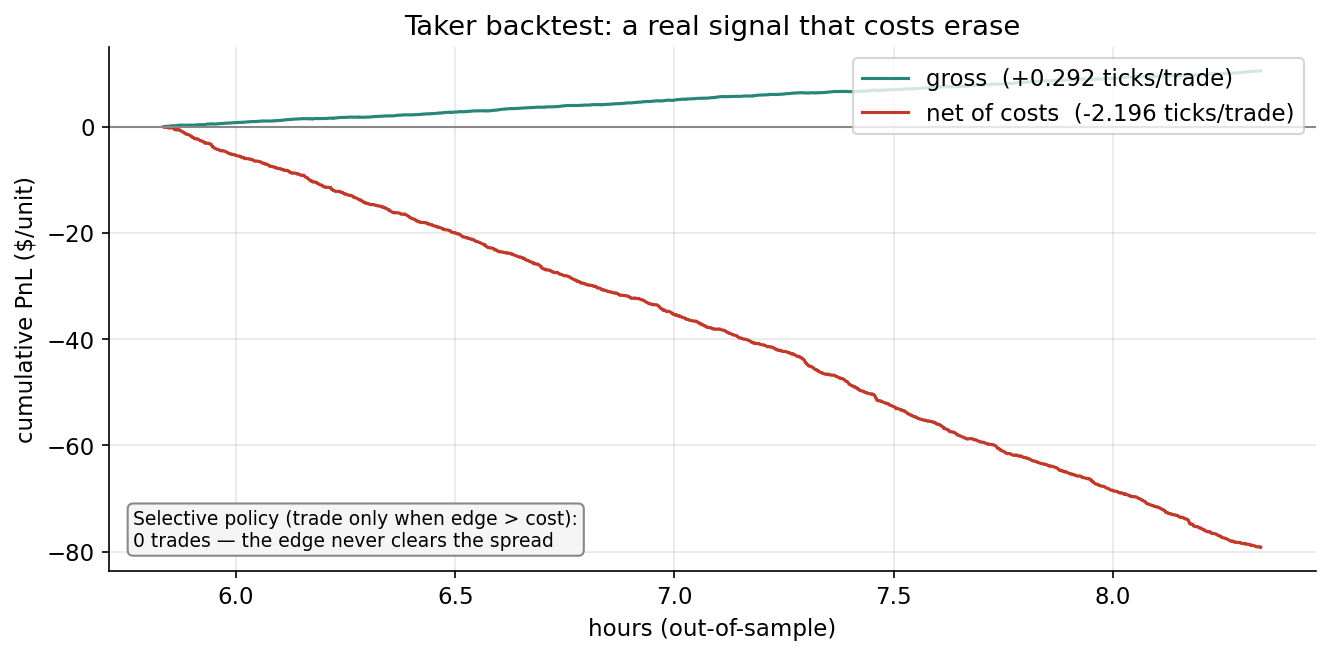
\includegraphics[width=\linewidth]{06_taker_backtest.png}
\caption{Out-of-sample taker backtest, gross and net of costs.}
\end{figure}

\section{Market making}

A market maker earns the spread but must control inventory and avoid being run over by
informed flow (Glosten and Milgrom, 1985). Plain Avellaneda-Stoikov quoting (Avellaneda
and Stoikov, 2008) bounds inventory but gives up most of the PnL; adding an OFI skew to
the reservation price uses the forecast to position inventory ahead of the move and
recovers the PnL at the same low inventory. Three policies are compared on the same
price path.

\begin{figure}[H]
\centering
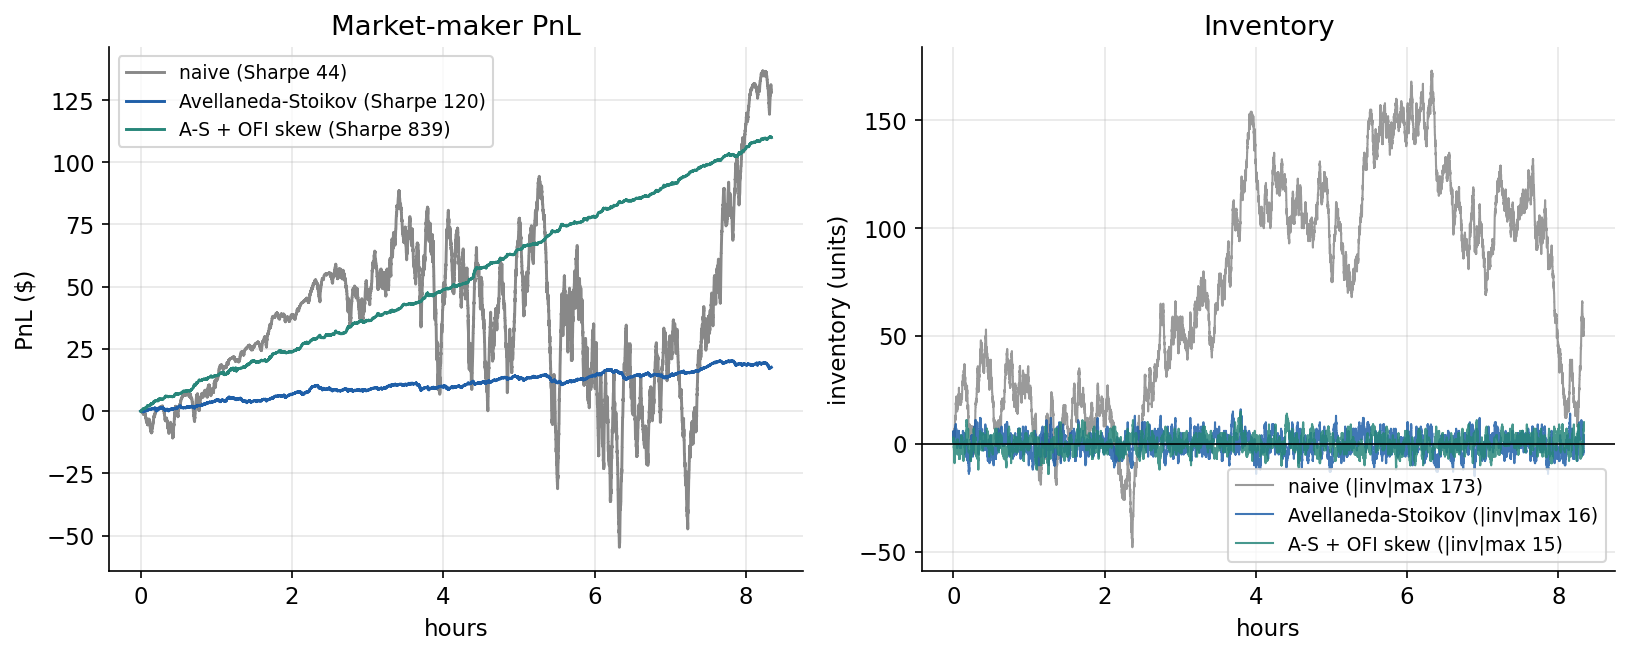
\includegraphics[width=\linewidth]{07_market_maker.png}
\caption{PnL (left) and inventory (right) for the three quoting policies.}
\end{figure}

\begin{table}[H]
\centering
\small
\begin{tabular}{L{3.6cm} c c c}
\toprule
\textbf{Policy} & \textbf{Final PnL} & \textbf{Max abs. inv.} & \textbf{Sharpe*} \\
\midrule
Naive symmetric     & \$128 & 173 & 44 \\
Avellaneda-Stoikov  & \$18  & 16  & 120 \\
A-S + OFI skew      & \$110 & 15  & 839 \\
\bottomrule
\end{tabular}
\end{table}

{\small *Sharpe is annualised from one-second marks and is large for all policies;
the meaningful comparison is across policies, not the absolute level.}

\section{Method and limitations}

Forecasting labels use the price move after OFI is observed, costs are charged at the
spread prevailing at trade time, and the model is fit on the training period and
evaluated on the test period. Standard errors use the Newey-West HAC estimator
(Newey and West, 1987) because high-frequency returns are autocorrelated.

The order book is a calibrated simulator; a live Binance collector is included so the
same pipeline can run on real data. The fill model is an Avellaneda-Stoikov intensity
rather than a queue-position simulation, and second-level Sharpe figures are not
comparable to fund-level Sharpes.

\section*{References}

\begin{reflist}
\item Avellaneda, M. and Stoikov, S. (2008). High-frequency trading in a limit order
      book. \emph{Quantitative Finance}, 8(3), 217-224.
\item Cont, R., Kukanov, A. and Stoikov, S. (2014). The price impact of order book
      events. \emph{Journal of Financial Econometrics}, 12(1), 47-88.
\item Glosten, L. R. and Milgrom, P. R. (1985). Bid, ask and transaction prices in a
      specialist market with heterogeneously informed traders. \emph{Journal of
      Financial Economics}, 14(1), 71-100.
\item Kyle, A. S. (1985). Continuous auctions and insider trading. \emph{Econometrica},
      53(6), 1315-1335.
\item Newey, W. K. and West, K. D. (1987). A simple, positive semi-definite,
      heteroskedasticity and autocorrelation consistent covariance matrix.
      \emph{Econometrica}, 55(3), 703-708.
\item Xu, K., Gould, M. and Howison, S. (2020). Multi-level order-flow imbalance in a
      limit order book. \emph{Market Microstructure and Liquidity}, 4(3-4).
\end{reflist}

\end{document}
